\documentclass[a4paper, 11pt]{article}

\usepackage{amsmath, amssymb, amstext, amsfonts, mathrsfs}	% Mathe
\usepackage{hyperref}		%Anklicken von Links
\usepackage[normalem]{ulem}	%weitere Formatierung von Schriften
\usepackage{fancyhdr}		%sch\"one Kopf- und Fußzeilen
\usepackage{verbatim}
\usepackage{graphicx}

\pagestyle{fancy}
\lhead{Data-driven intelegent systems\\}
\chead{\ \\Florian Vahl}
\rhead{\today\\}

\parindent0pt

\begin{document}
\section{Task}
\begin{figure}[h!] 
    \centering
    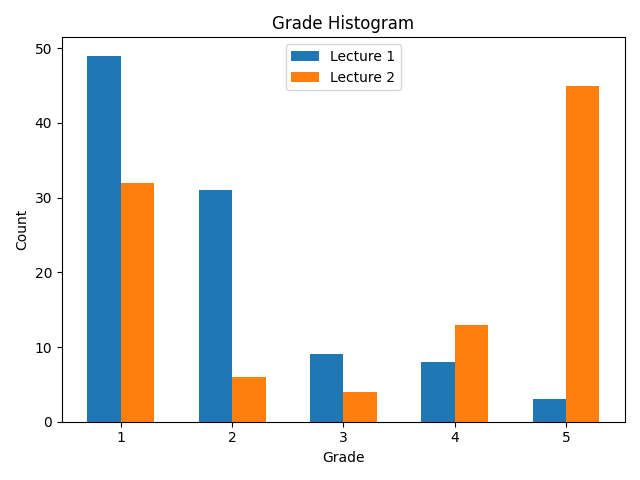
\includegraphics[width=\linewidth]{fig/Figure_1.png}
    \caption{This histogram shows a descete number of students for each given grade in two exams.}
    \label{fig:grades}
\end{figure}

Histogram in figure~\ref{fig:grades}

\begin{itemize}
    \item What are the characteristics of a histogram?

    This histogram shows how many instances exist for (in this case) each possible grade. It is also applicable for continuous values using bins, but the grades are descrete.

    \item Why do you think this plot was best to demonstrate the data?
    
    The histogram shows how many students have which grade for both exams. This opens the possibility for further manual analysis regarding the distribution of grades for each exam.
\end{itemize}

\newpage

\begin{figure}[h!] 
    \centering
    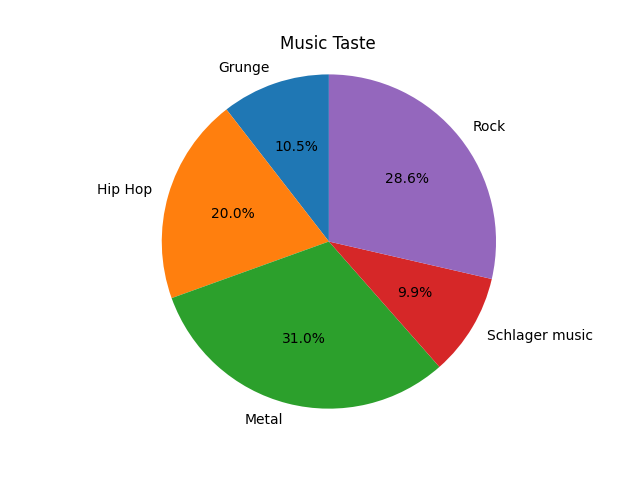
\includegraphics[width=\linewidth]{fig/Figure_2.png}
    \caption{This pie chart shows the music taste among 1000 asked people.}
    \label{fig:music}
\end{figure}

Music Pie Chart in figure~\ref{fig:music}

\begin{itemize}
    \item What are the characteristics of a pie chart?

    The pie chart shows the non overlapping classes as the partitions of a circle. 
    It gives an good overview of how set is splited into these classes and how it adds up. 
    It is not so practical for very big class size differences.

    \item Why do you think this plot was best to demonstrate the data?
    
    The given data was not overlapping and splitted the set of 1000 people into 5 classes which are good displayable on a pie chart. 
    It easily visualizes the size of each class in contrast to the total size and the other classes. 
\end{itemize}

\newpage

\begin{figure}[h!] 
    \centering
    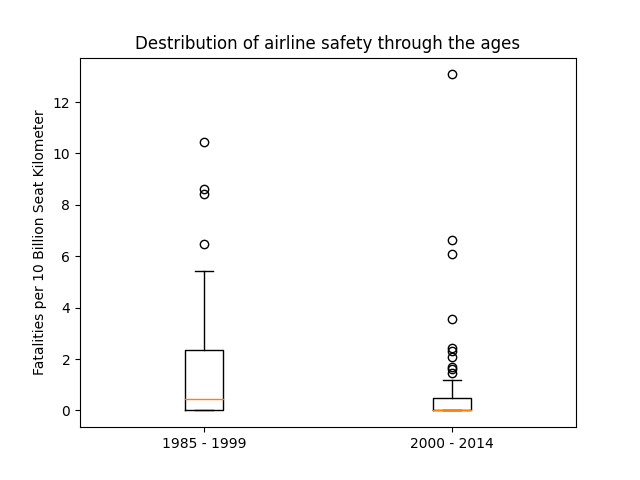
\includegraphics[width=\linewidth]{fig/Figure_3.png}
    \caption{This box plot shows the number of fatalaties per 10 billion seat kilometers for 57 airlines in the time from 1985-1999 and 2000-2015.}
    \label{fig:airline}
\end{figure}

Box plot in figure~\ref{fig:airline}

\begin{itemize}
    \item What are the characteristics of a box plot?

    The box plot shows the a box which represent the first and third quartile of the data, inside the box is a line which represents the median. 
    The 'T' like lines on the top and bottom of the box are the minimum and maximum values without outliers and the little circles are the outliers. 
    The box plot abstracts the data plot whithout hiding the distribution of the data like in a bar chart where only the mean is displayed.

    \item Why do you think this plot was best to demonstrate the data?
    
    In this case the fatalaties per (10 billion) seat kilometers is shown at two equal sized time intervals. 
    First of all the fatalaty values is corrected by the flown seat kilometers of the airline. This enshures a fair rating for bigger/smaller airlines. 
    This values are used in the box plot, where each data point represents one airline. 
    The box plot shows the mean fatalaties for all airlines in the two intervals, which is good to see the overall improvement over time in the two plot parts. 
    The plot also shows that not only the airlines got saver, there safety distribution is also narrowed in contrast to the first interval. 
    Showing the outliers displays the few critical airlines which could also be labeled and analyzed further more.
    All in all the plot summerizes the data from the 57 airlines with many data points in an smaller but informative plot.
\end{itemize}


\begin{figure}[h!] 
    \centering
    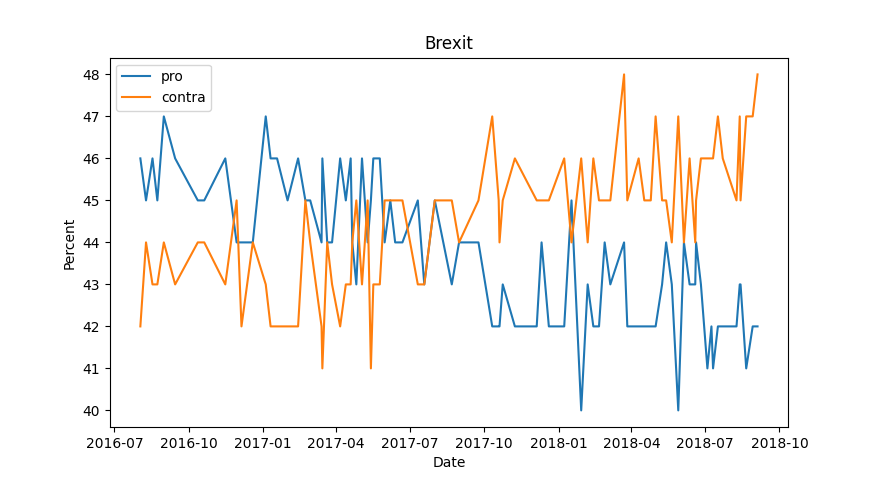
\includegraphics[width=\linewidth]{fig/Figure_4.png}
    \caption{This plot shows the percentage of people who think Brexit was wether right or wrong over time.}
    \label{fig:brexit}
\end{figure}

Plot in figure~\ref{fig:brexit}

\begin{itemize}
    \item What are the characteristics of this line plot?

    The plot shows the movement of the two values over time.

    \item Why do you think this plot was best to demonstrate the data?
    
    It nicely shows the pro and contra values throughout the time. Different events could be labeled in the plot.
\end{itemize}

\newpage

\begin{figure}[h!] 
    \centering
    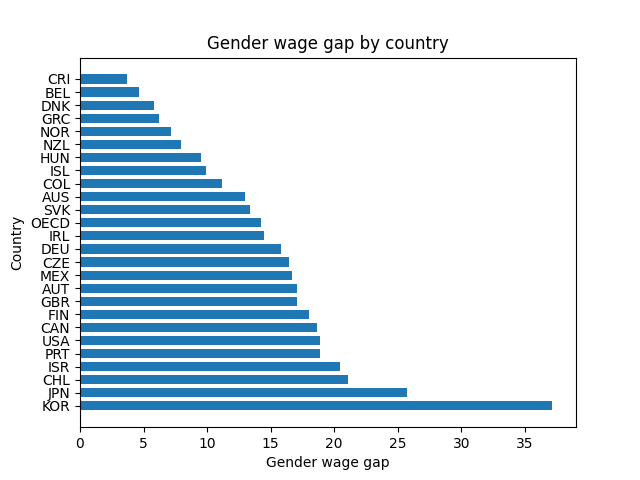
\includegraphics[width=\linewidth]{fig/Figure_5.png}
    \caption{This bar chart shows the deviation of wages for female employees with respect to wages for male employees determined by oecd for a number of countries.}
    \label{fig:gwg}
\end{figure}

Bar plot in figure~\ref{fig:gwg}

\begin{itemize}
    \item What are the characteristics of this line plot?

    It shows a value for each of the countries without furter information about e.g. the distribution.

    \item Why do you think this plot was best to demonstrate the data?
    
    It allows to compare the gab between the different countries, whitout beeing too big and confusing or losing e.g. the country data. 
\end{itemize}

\newpage

\section{Task}

\begin{itemize}
    \item Plot 1
    
    The data is not corrected by the amount of costline the states have and also a log scale would be nice to differentiate the small values without haveing a big spike.

    \item Plot 2
    
    The amount of medals shown does not scale with the emount of medals earned. The USA won nearly twice as many medals as Russia but have only one sixth more in this plot.

    \item Plot 3
    
    The number of cases seems to go down in 2016 but the plot only changes the time interval on the right side while still showing the absolute value of cases in this shorter time interval.
\end{itemize}

\newpage

\section{Task}

Notebook:

\begin{figure}[h!] 
    \centering
    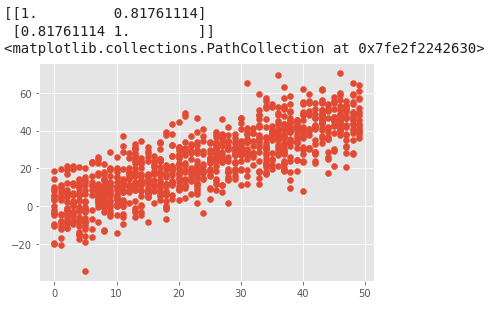
\includegraphics[width=\linewidth]{fig/corr1.png}
    \caption{The first correlation matrix shows a correlation 1 between (x, x) and also (y, y) (obviously). More interesting is the correlation cov of ~0.817 between x and y in both ways. It incicates that a bigger x value could imply a higher y value and the other way around.}
\end{figure}

\newpage

\begin{figure}[h!] 
    \centering
    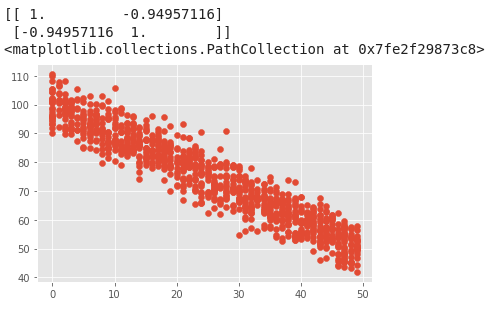
\includegraphics[width=\linewidth]{fig/corr2.png}
    \caption{The first correlation matrix shows a correlation 1 between (x, x) and also (y, y) (obviously). More interesting is the correlation cov of -0.949 between x and y in both ways. This indicates a negative correlation, so that a smaller x value results in a larger y value.}
\end{figure}

\newpage

\begin{figure}[h!] 
    \centering
    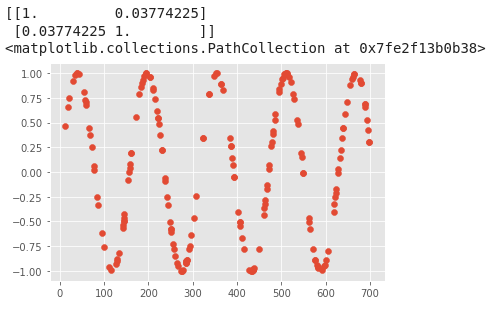
\includegraphics[width=\linewidth]{fig/corr3.png}
    \caption{The first correlation matrix shows a correlation 1 between (x, x) and also (y, y) (obviously). The non linear correlation can not be determined.}
\end{figure}

Chi-Square-Test:

\begin{table}[h!]
    \centering
    \begin{tabular}{ p{3cm}|p{4cm}|p{4cm}|p{2cm}}
        &Likes Zombie movies &Does not like Zombie movies&Total\\
        \hline
        Plays harp   & 24 (18)&6 (12)&30\\
        \hline
        Does ot play harp&8 (14)&16 (10)&24\\
        \hline
        Total&32&22&54\\
    \end{tabular}
    \caption{Table with completed values}
    \label{table:1}
\end{table}



There is $(I-1)*(J-1) = 1*1 = 1$ degree of freedom.

The $X^2$-Value is: $X^2 = \frac{(24-17.7)^2}{17.7} + \frac{(6-12.2)^2}{12.2} + \frac{(8-14.2)^2}{14.2} + \frac{(16-9.7)^2}{9.7} =\frac{1323}{110} \approx 12$.

For an $\alpha = 0.05  95\%$ of the values are below the threshold of $3,841$. Because $12$ is greater than $3,841$, the null hypothesis gets rejected and the data is propably corrected.
\newpage

\section{Task}

\begin{figure}[h!] 
    \centering
    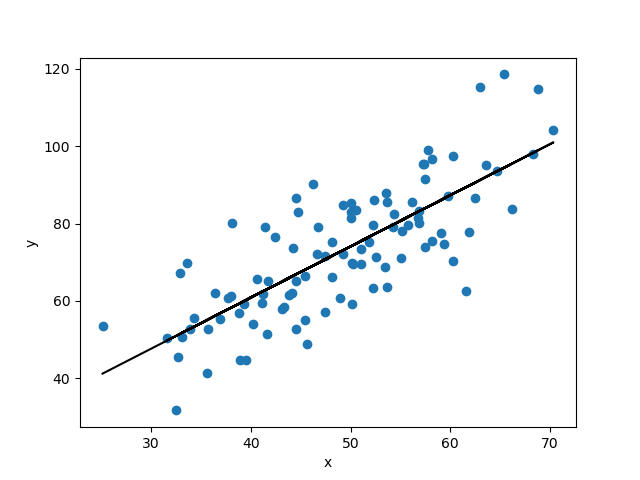
\includegraphics[width=\linewidth]{fig/regression.png}
    \caption{Line fitted in the data using the given regression method.}
    \label{fig:reg}
\end{figure}

\begin{itemize}
    \item Why is a regression also referred to as ordinary least square?
    
    Because the squared error beween the fitted line and the data points is minimal. 

    \item The regression results as seen in figure~\ref{fig:reg} are: 
    
    $\beta_1 = 1.322431022755357 \\ \beta_0 = 7.991020982270527$.

    In the model $\beta_1$ is the line slope of the fitted line and $\beta_0$ is the y-interception.

    \item For which data distribution a regression would not be a good fit?
    
    This given linear regression is not good for data that follows higher polinomial functions, exponential function or sinus like functions.

\end{itemize}

\newpage

\section{Code}

Github: 

\href{https://github.com/Flova/DAIS/blob/master/%C3%9Cbung%201/exercise1.py}{Plot Code}

\href{https://github.com/Flova/DAIS/blob/master/%C3%9Cbung%201/DAMI2_simpleRegression.py}{Regression Code}

\end{document}



















